\section{Ceasul DGT3000}
Ideal pentru efortul nostru de dezvoltare a proiectului ar fi să avem disponibile schema electrică și a PCB-ului aferente acestui ceas, însă din păcate nu avem la dispoziția noastră. Astfel, vom fi nevoiți să explorăm noi înșine modul în care acesta a fost construit și să extragem informațiile necesare. Mai jos se vor putea observa trei plăcuțe cu circuite imprimate și anume cea din partea superioară care este legată la clapetele ceasului (pentru a încheia tura curentă a jucătorului), cea din dreapta ce este conectata la mufa jack de 3.5 milimetri și cea principală din mijloc ce conține controller-ul (ca observație afișajul LCD se află pe partea dorsală a plăcuței). Putem afirma că acesta folosește un microcontroller pe 8 biți ST8L152M8 ce este legat la conectorul jack.

\begin{figure}[H]
	\centering
	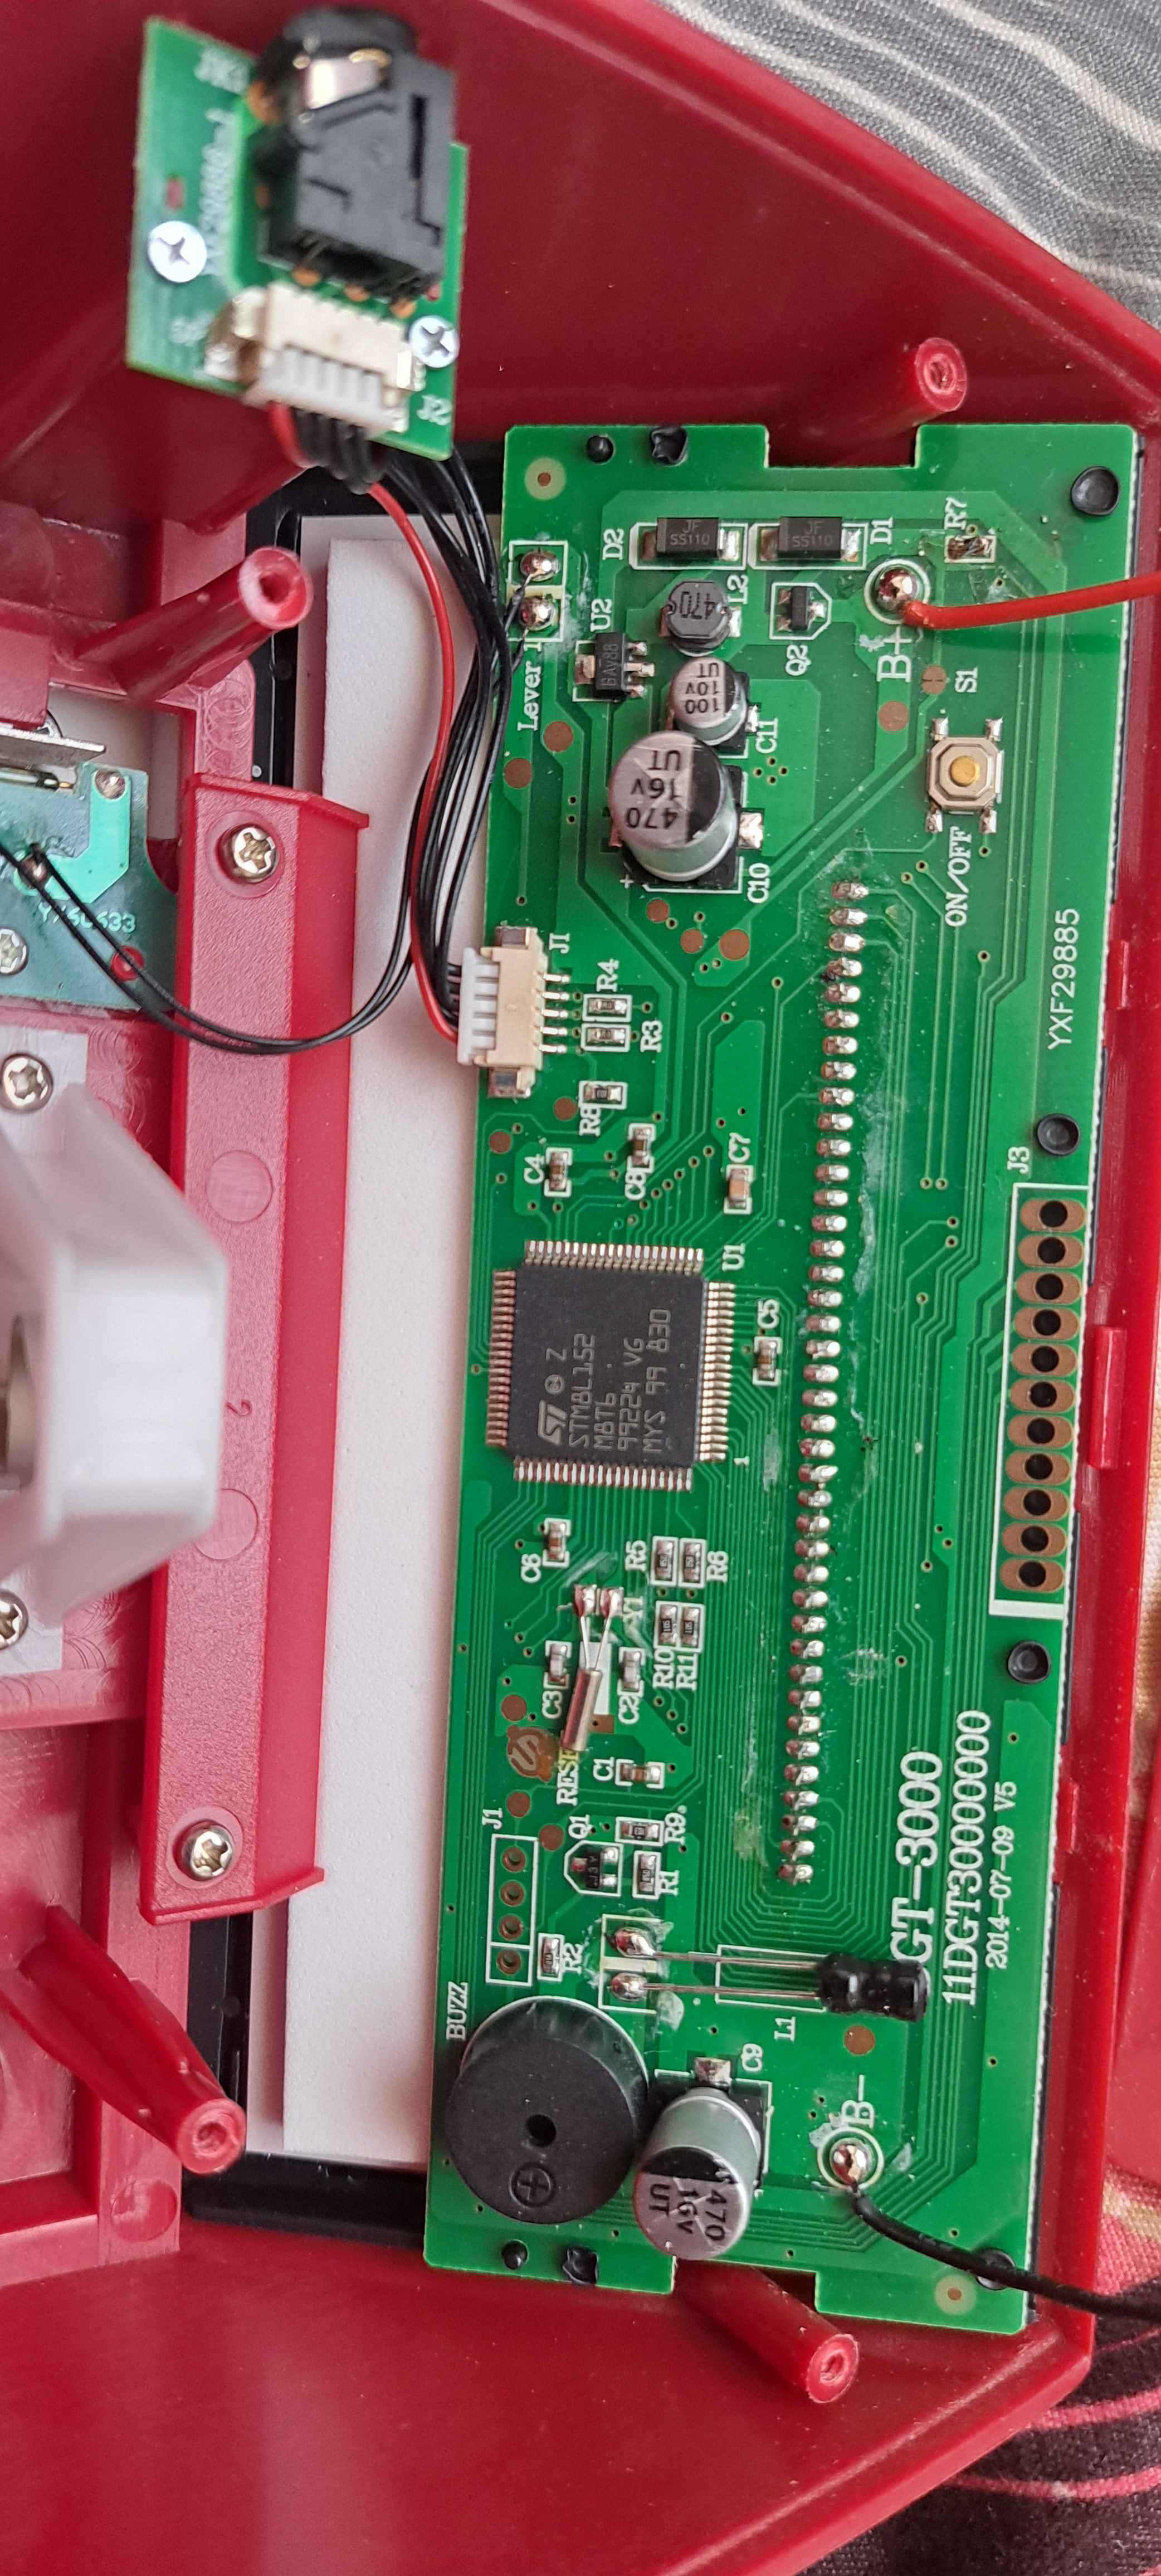
\includegraphics[width=0.5\textwidth, angle=-90]{../hw/clock_pcb.jpg}
	\caption{DGT3000 PCB}
\end{figure}
Bazat pe consultarea fișei de specificații a cipului și efectuarea unor teste de continuitate și tensiune s-au observat următoarele:
\begin{enumerate}
	\item În ciuda numărului de pini folosiți pentru conectorul jack de 3.5mm doar trei dintre acești prezintă conexiuni diferite (adică nu sunt legate unul la altul).
	\item Pinul 1 este legat la partea centrală a conectorului (Ring).
	\item Pini 2 și 3 sunt legați între ei iar apoi la vărful conectorului jack (Tip).
	\item Pinii 4 și 5 sunt legați între ei iar apoi la partea centrală a conectorului (Ring).
	\item Ajuns în circuitul principal pinul 1 este legat la SCLK din modulul SP1 al microcontroller-ului.
	\item Ajunși în circuitul principal pinii 4 și 5 sunt legați la masă.
\end{enumerate}